\section{Модальное управление по выходу.}

Исследуемая система описывается уравнениями:
\[
\begin{cases}
    \dot{x} = Ax + Bu, \\
    y = Cx + D,
\end{cases}
\]
где:
\begin{itemize}
    \item $x$ — вектор состояния системы,
    \item $u$ — входной сигнал (управление),
    \item $y$ — выходной сигнал.
\end{itemize}

Матрицы системы заданы следующим образом:

\[
A = \begin{bmatrix}
    5 & -7 & -5 & 1 \\
    -7 & 5 & -1 & 5 \\
    -5 & -1 & 5 & 7 \\
    1 & 5 & 7 & 5
\end{bmatrix}, \quad
B = \begin{bmatrix}
    5 \\
    7 \\
    1 \\
    9
\end{bmatrix}, \quad
C = \begin{bmatrix}
    0 & 0 & 2 & 2 \\
    1 & 1 & -1 & -1 \\
\end{bmatrix}
D = \begin{bmatrix}
    4 \\
    2 \\
\end{bmatrix}
\]


\subsection{Исследование наблюдаемости системы}

Для начала найдём матрицу наблюдаемости системы:
\[
V = \begin{bmatrix}
    C \\
    CA \\
    CA^2
\end{bmatrix} =
\begin{bmatrix}
    1 & 0 & 2 \\
    4 & -3 & 2 \\
    -11 & -6 & 16
\end{bmatrix}.
\]
Ранг матрицы наблюдаемости $V$ равен 3. Согласно критерию Калмана, система является \textbf{полностью наблюдаемой}, так как ранг матрицы наблюдаемости равен порядку системы.

Найдём собственные числа матрицы $A$:
\[
\sigma(A) = \{-8, 4, 8, 16\}.
\]

\subsection{Синтез наблюдателя и регулятора}

Выберем следующие спектры для наблюдателя и регулятора, которые обеспечат асимптотическую устойчивость замкнутой системы:
\[
\sigma(G_{\text{ctrl}}) = \{-1, -3, -3, -3\}, \quad
\sigma(G_{\text{obsv}}) = \{-1, -3, -3, -3\}.
\]

Используя метод синтеза регулятора и наблюдателя через уравнения Сильвестра, получим следующие матрицы $K$ и $L$:

\[
G_{\text{ctrl}} = \begin{bmatrix}
    -1 & 0 & 0 & 0 \\
    0 & -3 & 1 & 0 \\
    0 & 0 & -3 & 1 \\
    0 & 0 & 0 & -3
\end{bmatrix}, \quad
Y = \begin{bmatrix}
    1 \\
    1 \\
    1 \\
    1
\end{bmatrix}^T, \quad
K = \begin{bmatrix}
    8.51 \\
    -8.91 \\
    -0.87 \\
    -1.36
\end{bmatrix}^T.
\]

\[
G_{\text{obsv}} = \begin{bmatrix}
    -1 & 0 & 0 & 0 \\
    0 & -3 & 1 & 0 \\
    0 & 0 & -3 & 1 \\
    0 & 0 & 0 & -3
\end{bmatrix}, \quad
Y = \begin{bmatrix}
    1 & 1 \\
    1 & 1 \\
    0 & 0 \\
    1 & 1
\end{bmatrix}, \quad
L = \begin{bmatrix}
    35.60 & 35.60 \\
    -38.39 & -38.39 \\
    -12.02 & -12.02 \\
    -15.18 & -15.18
\end{bmatrix}.
\]

\subsection{Проверка корректности синтеза}

Вычислим собственные числа матриц регулятора $(A + BK)$ и наблюдателя $(A + LC)$:

\subsubsection{Собственные числа наблюдателя}
\[
    \sigma(A + LC) \approx \{-1, -3.0005, -2.9997 \pm 0.0004i\}.
\]

\subsubsection{Собственные числа регулятора}
\[
    \sigma(A + BK) \approx \{-1, -3.9996, -4.0002 \pm 0.0004i\}.
\]

Спектры практически совпадают с заданными, за исключением незначительных погрешностей. Это подтверждает корректность синтеза как регулятора, так и наблюдателя.


\subsection{Моделирование системы}

Проведём моделирование системы с начальными условиями:
\begin{itemize}
    \item Вектор состояния системы: $x(0) = \begin{bmatrix} 1 & 1 & 1 & 1 \end{bmatrix}^T$.
    \item Вектор состояния наблюдателя: $\hat{x}(0) = \begin{bmatrix} 0 & 0 & 0 & 0 \end{bmatrix}^T$.
\end{itemize}

\begin{figure}[H]
    \centering
    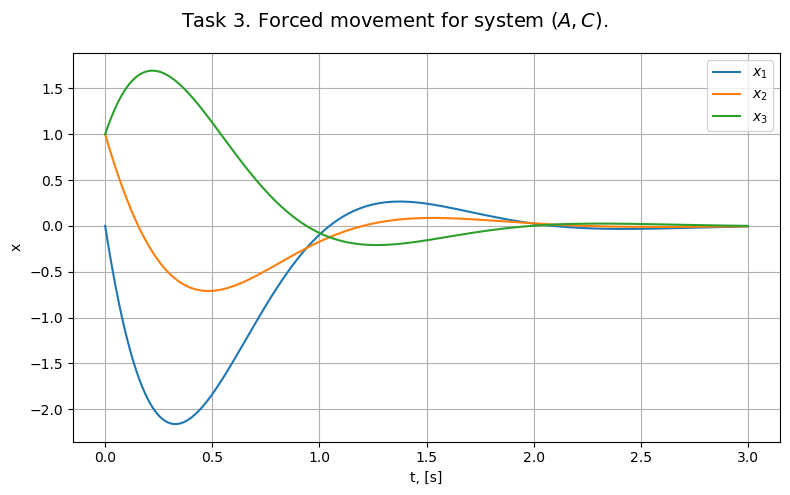
\includegraphics[width=0.7\textwidth]{../../plots/task_3_1.png}
    \caption{Состояние системы}
    \label{fig:task_3_state_system}
\end{figure}

\begin{figure}[H]
    \centering
    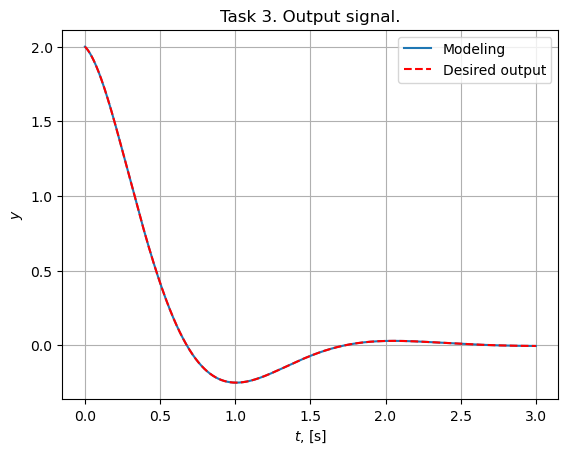
\includegraphics[width=0.7\textwidth]{../../plots/task_3_2.png}
    \caption{Ошибка сходимости}
    \label{fig:task_3_error_system}
\end{figure}

\begin{figure}[H]
    \centering
    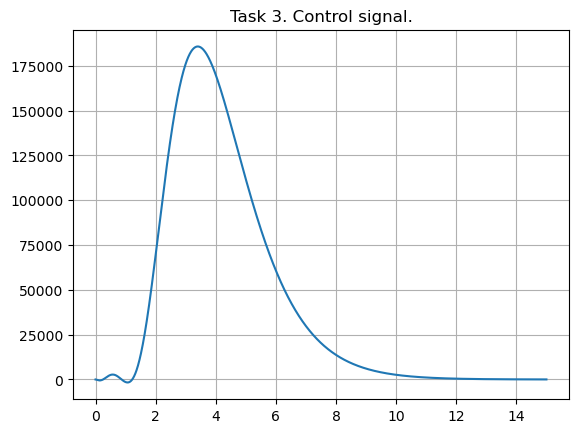
\includegraphics[width=0.7\textwidth]{../../plots/task_3_3.png}
    \caption{Управление регулятора}
    \label{fig:task_3_control_signal}
\end{figure}


\subsection{Вывод}
В рамках данного задания мы синтезировали \textbf{полное управление по выходу}, которое включает связку наблюдателя и регулятора. Мы работали с системой, которая является \textbf{полностью наблюдаемой и управляемой}, что позволило нам свободно выбирать желаемые спектры как для наблюдателя, так и для регулятора. Проведённое моделирование подтвердило успешную работу связки: наблюдатель корректно оценивал состояние системы, а регулятор обеспечивал стабилизацию системы в соответствии с заданными требованиями.